% !TEX root = ../Survey.tex
	We now discuss  labeling schemes for the function \NCA. 
	Two variants of labeling schemes that support  the  function appear in the literature, \NCAl and \NCAf explained hereafter.
Suppose a tree $T=(V,E)$ has a predefined label assignment of $\log n$ bits  from a preset name domain, and denote  the product of such an  assignment for a  node $v \in V$  as the \emph{node identifier} of  $v$, or simply $\Id(v)$.  We can extend all labeling schemes presented so far to support node identifiers  by modifying their encoder to concatenate the node identifier to each label. In the case of \NCA such an extension is not as straightforward since it should return, for two nodes in the tree, the node identifier of  a third node.  We treat both variants, and denote labeling schemes for \NCA specifically designed to support node identifiers as \NCAf, and those that do not as  \NCAl.

In Section~\ref{sec:Lit-NCA} we provide  a literature overview and describe connections to related problems. In Section~\ref{sec-NCA-FIXED} we survey a  connection between \NCAf and the functions \distance,  \seplevel~ and \centerf. The connection leads to a lower bound, for which an asymptotically identical upper bound is presented. We  dedicate  Section~\ref{section-NCA-designer}  to the  construction of a \NCAl labeling scheme, of the same asymptotic size.
We then show how to improve  this labeling scheme to achieve labels of size $O(\log n)$. Finally, we  discuss  an  extension  of labeling schemes that  provides  a natural bridge between the two variants.

\subsection{Literature review}\label{sec:Lit-NCA}
The problem of finding nearest (occasionally referred, least) common ancestors (NCAs) is non-trivial already in the non-distributed setting. 
Its importance is derived by its role as a subroutine of common algorithms for minimum spanning trees in a graph, finding maximum weighted matching in a graph, and bounded tree-width algorithms.
Aho, Hopcroft and Ullman~\shortcite{aho} were among the first to consider the problem of finding NCAs, and \citeN{hareltarjan} were the first to describe an algorithm that uses only linear time and space for pre-processing and can answer \NCA queries in constant time.
Their algorithm is distributed for complete binary trees, but uses a non-distributed, precomputed auxiliary data structure in order to generalise the results to arbitrary trees.
A more recent,  simpler, and  distributed algorithm was presented by \citeN{Alstrup02NCA} in the form of a \NCAl labeling scheme of size $10 \log n+O(1)$.  The labeling scheme was improved recently by~\citeN{Green14} to $3 \log n+O(1)$, along with a lower bound of $1.008n$, and a  non-constructive proof of a labeling scheme of size $2.772 \log n +O(1)$.
 
 \citeN{peleg2000informative} showed that  for \NCAf  labels of size $\Theta(log^2 n)$ are sufficient and required.
\citeN{blin2010fast} extend Alstrup et al.'s labeling scheme for labels of length bound by constant $k$.
 Experimental studies of  labeling schemes for the function are considered in~\cite{caminiti2009informative,Fischer09}.
~\citeN{Korman07K} studied \NCAf on a different model called  \emph{1-query}. In this model, the decoder has access to a \emph{query} function, that gets two labels and returns  a node identifier.  In this setting  \NCAf queries can be answered using labels of size  $O(\log n)$.
			
\paragraph{Connection to other problems}
The function \NCA  is tightly related to two problems.
First,  finding a nearest common ancestor labeling scheme is equivalent to the \emph{discrete range searching problem}~\cite{gabow}.
Second, for both \NCAf and \NCAl, the  labels produced can determine ancestry relation directly. 
Put formally, any labeling scheme $\tuple{e,d}$  supporting the  \NCA function computes a label assignment $e_T$  with following property:
For $u,v \in T$, we can construct a decoder that receives $\la(u),\la(v)$  determines ancestry.
The decoder may use the \NCA decoder $d$ and compare the result to $\la(u)$. If $u$ is a parent of $v$, the two are equivalent and our ancestry decoder may safely return \emph{True}.
As a result, any lower bounds that apply to ancestry labeling schemes apply to NCA schemes as well.
A last connection between  the function \NCA and routing is discussed in Section~\ref{section-NCA-designer}.

\subsection{\NCAf} \label{sec-NCA-FIXED}
In this section, we present lower and upper bounds for \NCAf.
	\subsubsection{\NCA, \seplevel, and their connection to \distance }
		\citeN{Peleg05} proved that  $\Omega(\log^2 n)$ bits are necessary for any \NCAf labeling scheme, as well as the functions \seplevel, and \centerf.
		Recall that the function \seplevel returns the length of the path  $r \leadsto w $ in $T$ where $r$ is the root and $w$ is $NCA_T(u,v)$.
			\begin{theorem} \cite{Peleg05}\label{NCAconnection}
			For  labeling schemes  on $Trees(n)$, we have the following claims:
			\mbox{}
			\begin{enumerate}
						\item Given an  $f(n)$ \distance labeling scheme, we can construct a $f(n)+\log n$-\seplevel labeling scheme.
			\item Given an  $f(n)$ \seplevel labeling scheme, we can construct a $f(n)+\log n$-\distance labeling scheme.
			\item Let g(n) denote the maximum size of an identifier of any node in $Trees(n)$. If an \NCAf labeling scheme has labels of size at most  $l(n) \cdot g(n)$ then  there exist a \seplevel labeling scheme of size  $ l(n) \cdot (g(n) + \log n).$ 
			\end{enumerate}
			\end{theorem}
			\begin{proof}
			To prove Claim 1, assume there exist a distance labeling scheme  $\tuple{e_{dist},d_{dist}}$. 
			The encoder  $e_{dist}$ computes a label assignment  for a tree  $T$ rooted in $r$ with nodes $u$, $v$ and $w$ such that  $w= \NCA(u,v)$.
			We transform the encoder $e_{dist}$ by concatenating a prefix  $\depth(v)$
			\footnote{ Section~\ref{definitions-of-trees}): A node $v$ in a tree $T=(V,E)$ rooted in $r$ has  $\depth(v)$  edges on the path $r \leadsto v$.}  to the label $\la(v)$ assigned by $e_{dist}$ to every $v \in V$, using additional  $\log n$ extra bits.
			The decoder can now compute \seplevel$(u,v)$, by   observing that 
			$\distance(u,v) = \distance(u,\NCA(u,v))+\distance(v,\NCA(u,v)) \text{, and } \depth(u)=\depth(\NCA(u,v))+\distance(u,\NCA(u,v))$
			 (the same formula holds by replacing $u$ with $v$).
			 It follows that  $$\depth(\NCA(u,v)) =  \frac{\depth(u)+\depth(v)-dist(u,v)}{2} = \seplevel(u,v).$$
			 We prove Claim 2  using the same transformation, i.e. adding $\depth(v)$	 to all labels produced by the encoder of any \seplevel labeling scheme.  
			 We prove Claim 3  by the same transformation, with the exception that  the new encoder adds $\depth(v)$ to the node identifier, adding exactly $\log n$ for  each of the node identifiers.
			\end{proof}
			
			\distance labeling scheme has a lower bound of $\Omega(\log^2 n)$ on the size of the label~\cite{gavoillea2004distance}.
			Assume that there exist a labeling scheme for \NCAf  of size $\phi(n) = o(\log^2(n))$. Since $g(n) = \log n$, it implies that $l(n) = o(\log n)$.
			By Claim 3, there also  exist a corresponding labeling scheme for \seplevel of size $o(\log^2 n)$.
			That labeling scheme, by  Claim 2, leads to a distance labeling scheme for distance of size $o(\log^2 n)$, in contrast with the lower bound mentioned~\cite{gavoillea2004distance}.
			
			\begin{corollary}
			Any labeling scheme supporting \NCAf for $Trees(n)$ must use labels of size $\Omega(\log^2(n))$.
			\end{corollary}
			 
\subsubsection{Upper bound for \NCAf}
It remains to prove that  there exist an \NCAf  matching (asymptotically) the lower bound.		 
For brevity, we repeat the definitions related to heavy-light decomposition (Section~\ref{tec:heavylight}):

$\hchild(v)$ is the (unique) heavy child of $v$,
$\lchildren(v)$ is the set of light children of $v$,
$\lsize(v)$ is the weight of $v$ not including the tree rooted in its heavy child,
$\lpath(v)$ is the list of all light nodes in  $r \leadsto v$,
$\ldepth(v) = \vert \lpath(v) \vert$,
$\hpath(v)$ is the set  of nodes on the same heavy path as $v$.


	\begin{theorem}\label{NCA-fixed-upper} \cite{Peleg05}
	There exist an \NCAf labeling scheme with labels of size at most $O(\log^2 n)$.
	\end{theorem}

	\begin{proof}
	Let  $T$  be a tree rooted in  $r$, where every node  $v \in V$ with light depth  $\ldepth(v)$ has   a unique  predefined identifier, $\Id(v)$.
%	 As proved in Section~\ref{tec:heavylight},  there are $1 \leq \ldepth(v) \leq \log n$ light nodes on  path between the root and any node  $v$ in $T$. 
 The label of node $v \in T$ is  defined as a concatenation of two parts, namely, $\mathcal{C}_a(v)$ and $\mathcal{C}_b(v)$ defined below.
	 
	 $\mathcal{C}_a(v)$   contains $\Id(v)$, and  an ancestry label as defined in Section~\ref{section:NaiveAncestry}, using at most $2 \log n $ bits, and in total at most $3 \log n $ bits.
	  $\mathcal{C}_b(v)$  contains a  concatenation (Section~\ref{section:Misc-Tools}) of triplets  of the form $\tuple{\Id(l_i),\Id(n_i),d_i}$, for $ 1 \leq i \leq  ldepth(v)$, where 
	 $l_i$  is the $i$'th light node in $\lpath(v)$, $d_i$ is the depth of $l_i$,  and $n_i$ is the node adjacent to $l_i$ on  $ r \leadsto l_i$.
	 Each triplet requires at most $3 \log n$ bits, and thus  $\mathcal{C}_b$ contains at most $3\log^2 n$ bits.
	 In conclusion, for every node $v \in T$,  $\vert \la(v) \vert = \vert \mathcal{C}_b(v) \vert  + \vert \mathcal{C}_a(v) \vert \leq 3(\log^2 n+ \log n)$.
	 
	We describe the operation on two nodes $u,v \in T$ with NCA $w$.
	The decoder  uses $\mathcal{C}_a$  to determine if one is an ancestor of the other, and if so returns its node identifier.
	At this point we can safely claim that  the path $u \leadsto v$ traverses exactly two  of $w$'s edges, where at least one of those  must be a light edge (see Figure~\ref{fig:NCAPeleg} for a demonstration).
	Thus, the decoder computes the common prefix of $\mathcal{C}_b(u)$ and $\mathcal{C}_b(v)$, and determines the first  $k$ for which the $k$'th triplet in $\mathcal{C}_b(u)$  is not equal to the $k$'th triplet in $\mathcal{C}_b(v)$.
	Since each triplet contains the depth of the light node it represents, we can deduce which of them is closer to $w$, and if the depth is equal we choose one arbitrarily.
	We  return the parent of the light node, stored in the selected triplet. 
	\end{proof}
	
					\begin{figure}[!ht] 
				\centering
				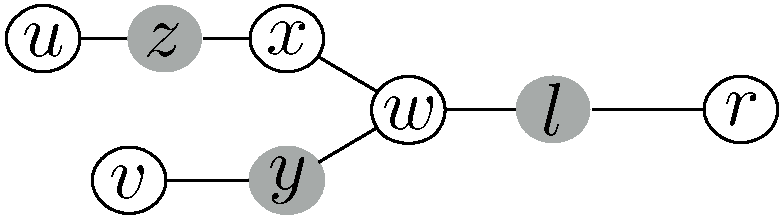
\includegraphics[width=60mm]{./Figures/NCApeleg.pdf}
				\caption{The nearest common ancestor w=\NCA(u,v) in a root rooted in r. The node  l is the last light node in common in the paths $r \leadsto u$ and $r \leadsto v$, and  $y$ and $z$ are the first light nodes immediately after $l$ on those paths, where $depth(z)>depth(y)$. Straight lines represent edges, dashed lines are paths, and grey nodes are light nodes. }
				\label{fig:NCAPeleg}
			\end{figure}
			
\subsection{\NCAl}\label{section-NCA-designer}
		We prove that there exist a \NCAl  labeling scheme of size  $O(\log n)$ in two steps.
		First, we present a simple (inefficient) labeling scheme with $O(\log^2 n)$  and then we prove that by a slight improvement, the label size decreases to $O(\log n)$. 
		 The first labeling scheme is by itself a modified version of the one presented in Theorem~\ref{NCA-fixed-upper}.
		Rather than storing the light path for every node along with the node above it, we store the light path along with the distance of the heavy paths  between each two consecutive light nodes. 
		\begin{theorem}\label{thm:nca-designer-long}
		There exist a \NCAl labeling scheme $\tuple{e,d}$ with label size bounded by $O (\log^2 n)$.
		\end{theorem}
		\begin{proof}
		Let $T=(V,E)$ be a tree rooted in $r$. For convenience,  $r$ is a heavy node with the  label $0$.
		We first compute a heavy-light decomposition of $T$ (Section~\ref{tec:heavylight}).

		The  new label   comprises the concatenation of the tuples  $\tuple{h_i,l_i}$, where $l_i$ is the index of  $i$'th light node  in $\lpath(v)$, and $h_i$ is the (possibly null) length of the heavy path $\hpath(l_i)$,  from $l_{i-1}$ to $l_i$ or to $v$ when $i=\ldepth(v)$.
		 See Figure~\ref{fig:NCAESBEN} for an illustration.
		 
		Since $1 \leq h_i, l_i \leq n$, each tuple requires at most  $2 \log n$ bits.
		Since $\vert \lpath(v) \vert \leq \log n$ (Section~\ref{tec:heavylight}), the total label size is bounded by $2\log^2 n$.
		To complete the proof we show how to compute the label of the NCA of two nodes $u$ and $v$ with labels $\la(u)= h_1^u,l_1^u \dots h_k^u,l_k^u$ and $\la(v) =  h_1^v,l_1^v \dots h_{k'}^v,l_{k'}^v $ respectively.
		 Without loss of generality assume that $k \leq k'$.
		We find the first $i$ for which $h_i^u,l_i^u \neq  h_i^v,l_i^v$.
		If there is no such $i$, then $u$ is the ancestor of $v$ and we return its label.
		 If $h_i^u = h_i^v$    we return the label $h_1^u,l_1^u \dots h_i^u$.
		 Otherwise, we return $h_1^u,l_1^u \dots  min\{h_i^u,h_i^v\}$.
		
		 \end{proof}	
		 
		 Note that this labeling scheme can return the depth of the NCA, in other words the \seplevel.
		 By Theorem~\ref{NCAconnection}, any   labeling scheme supporting \seplevel must have labels of size $\Omega(\log^2 n)$.
	 Moreover, using the formulas from Theorem~\ref{NCAconnection}  we observe that the function  \distance may also be computed using these labels.
		The first labeling scheme for the function \distance~\cite{Peleg00} uses separator decomposition.
		The label created in this labeling scheme  can not be used to determine the  functions \NCA, \adjacency and \ancestry.
		 In contrast, our  labeling scheme  stores enough information on the topology of the tree to determine all(!) the functions surveyed on trees.
		 
		The  labeling scheme presented is based on the ability  to choose a node's name. The one presented next utilises the ability further, and reduces the bound on the label size from $O(\log^2 n)$  to $O (\log n)$.
		\subsubsection{\NCAl with $O(\log n)$ bits}
		The maximum label size in Theorem~\ref{thm:nca-designer-long} is the longest description  of a sequence of at most $\log n$ tuples of the form $\tuple{h_i,l_i}$.
		 We do not  consider  assigning short labels to nodes with big size, nor do we account for the total length possible for the heavy paths.
		 However, even with those improvements, we will still be able to determine \seplevel, which implies a label of size $\Omega(\log^2 n)$ as mentioned.
		 
		 The key observation is that the function \NCA can be  determined even without knowing the exact length of the heavy paths.
		 We only require that each label of the nodes on a heavy path  $h_1 \dots h_k$ has a total order on that path, i.e., given two labels, determine which of them is first on the path.
		 Alstrup, Gavoille, Kaplan and Rauhe~\shortcite{Alstrup02NCA}  use those two  observations  as well as   Lemma~\ref{lemma:Gilbert}  to construct  a $O(\log n)$  \NCAl  labeling scheme presented below.

		\begin{theorem}\cite{Alstrup02NCA}\label{thm:nca-short}
		There exist a \NCAl labeling scheme  of  size  $O (\log n)$.
		\end{theorem}
		
		\begin{notproof}[Sketch]
		Consider a node $v$ where $parent(v)= u$ in a tree $T$ rooted in $r$ with $\ldepth(v) =k$ and  $\lpath= \{ lp_1 \dots lp_k \}$.
		The label  comprises the concatenation of the tuples  $\tuple{h'_i,l'_i}$.
		We first construct the labels given by  Theorem~\ref{thm:nca-designer-long} as auxiliary labels where   $\tuple{h_i,l_i}$  defined as in Theorem~\ref{thm:nca-designer-long}.
		
		To compute each $l'_i$, we use Lemma~\ref{lemma:Gilbert} with   $\size(lp_i)$ and the $\lsize$ of each of its  \emph{siblings}  in $T$.
		The lemma provides $l'_i$ a  label appropriate to $\size(lp_i)$, and more precisely:    
		$$\vert l'_i \vert  \leq  \log \size(v) -  \log \lsize(p(lp_i)) +1,$$
		where $p(lp_i)$ is the parent of $lp_i$.
		
		To compute each $h'_i$ we use  Lemma~\ref{lemma:Gilbert} with  the size of all nodes on the heavy path rooted in $lp_i$, $\hpath(v)$, ordered by their depth.
		That is, since we want to have labels as small as possible the closer we are to $lp_i$.
		The lemma provides $h'_i$ a  label appropriate to the light size of the $h_i$'th node on  $\hpath(v)$. More precisely:    
		$$\vert h'_i \vert \leq \log\size(lp_{i}) - \log\lsize(v) +1.$$
		
		In contrast to the previous labeling scheme, both $l'_i$ and $h'_i$ have variable size. In order to distinguish the different parts in $\la(v) = h'_1,l'_1, \dots h'_k,l'_k$ we use a separating string (Section~\ref{section:Misc-Tools}), which doubles the size of the label.
		By induction,  it can be shown that $\vert h'_1 \vert, \vert l'_1 \vert, \dots  \vert h'_k \vert ,\vert l'_k \vert  \leq \log n +4k +2$. The proof is similar to that of Lemma~\ref{lemma:tikun}.
		
		The decoder is computed similarly to the one defined in Theorem~\ref{thm:nca-designer-long} with the exception that in the last case we use  $\min_{\lex}\{h_i,h_i'\}$ instead of $\min{\{h_i,h_i'\}}$.
		
		For proof of the induction, and the correctness  of the decoder, see~\cite{Esben13}.
		\end{notproof}


					\begin{figure}[!ht] 
				\centering
				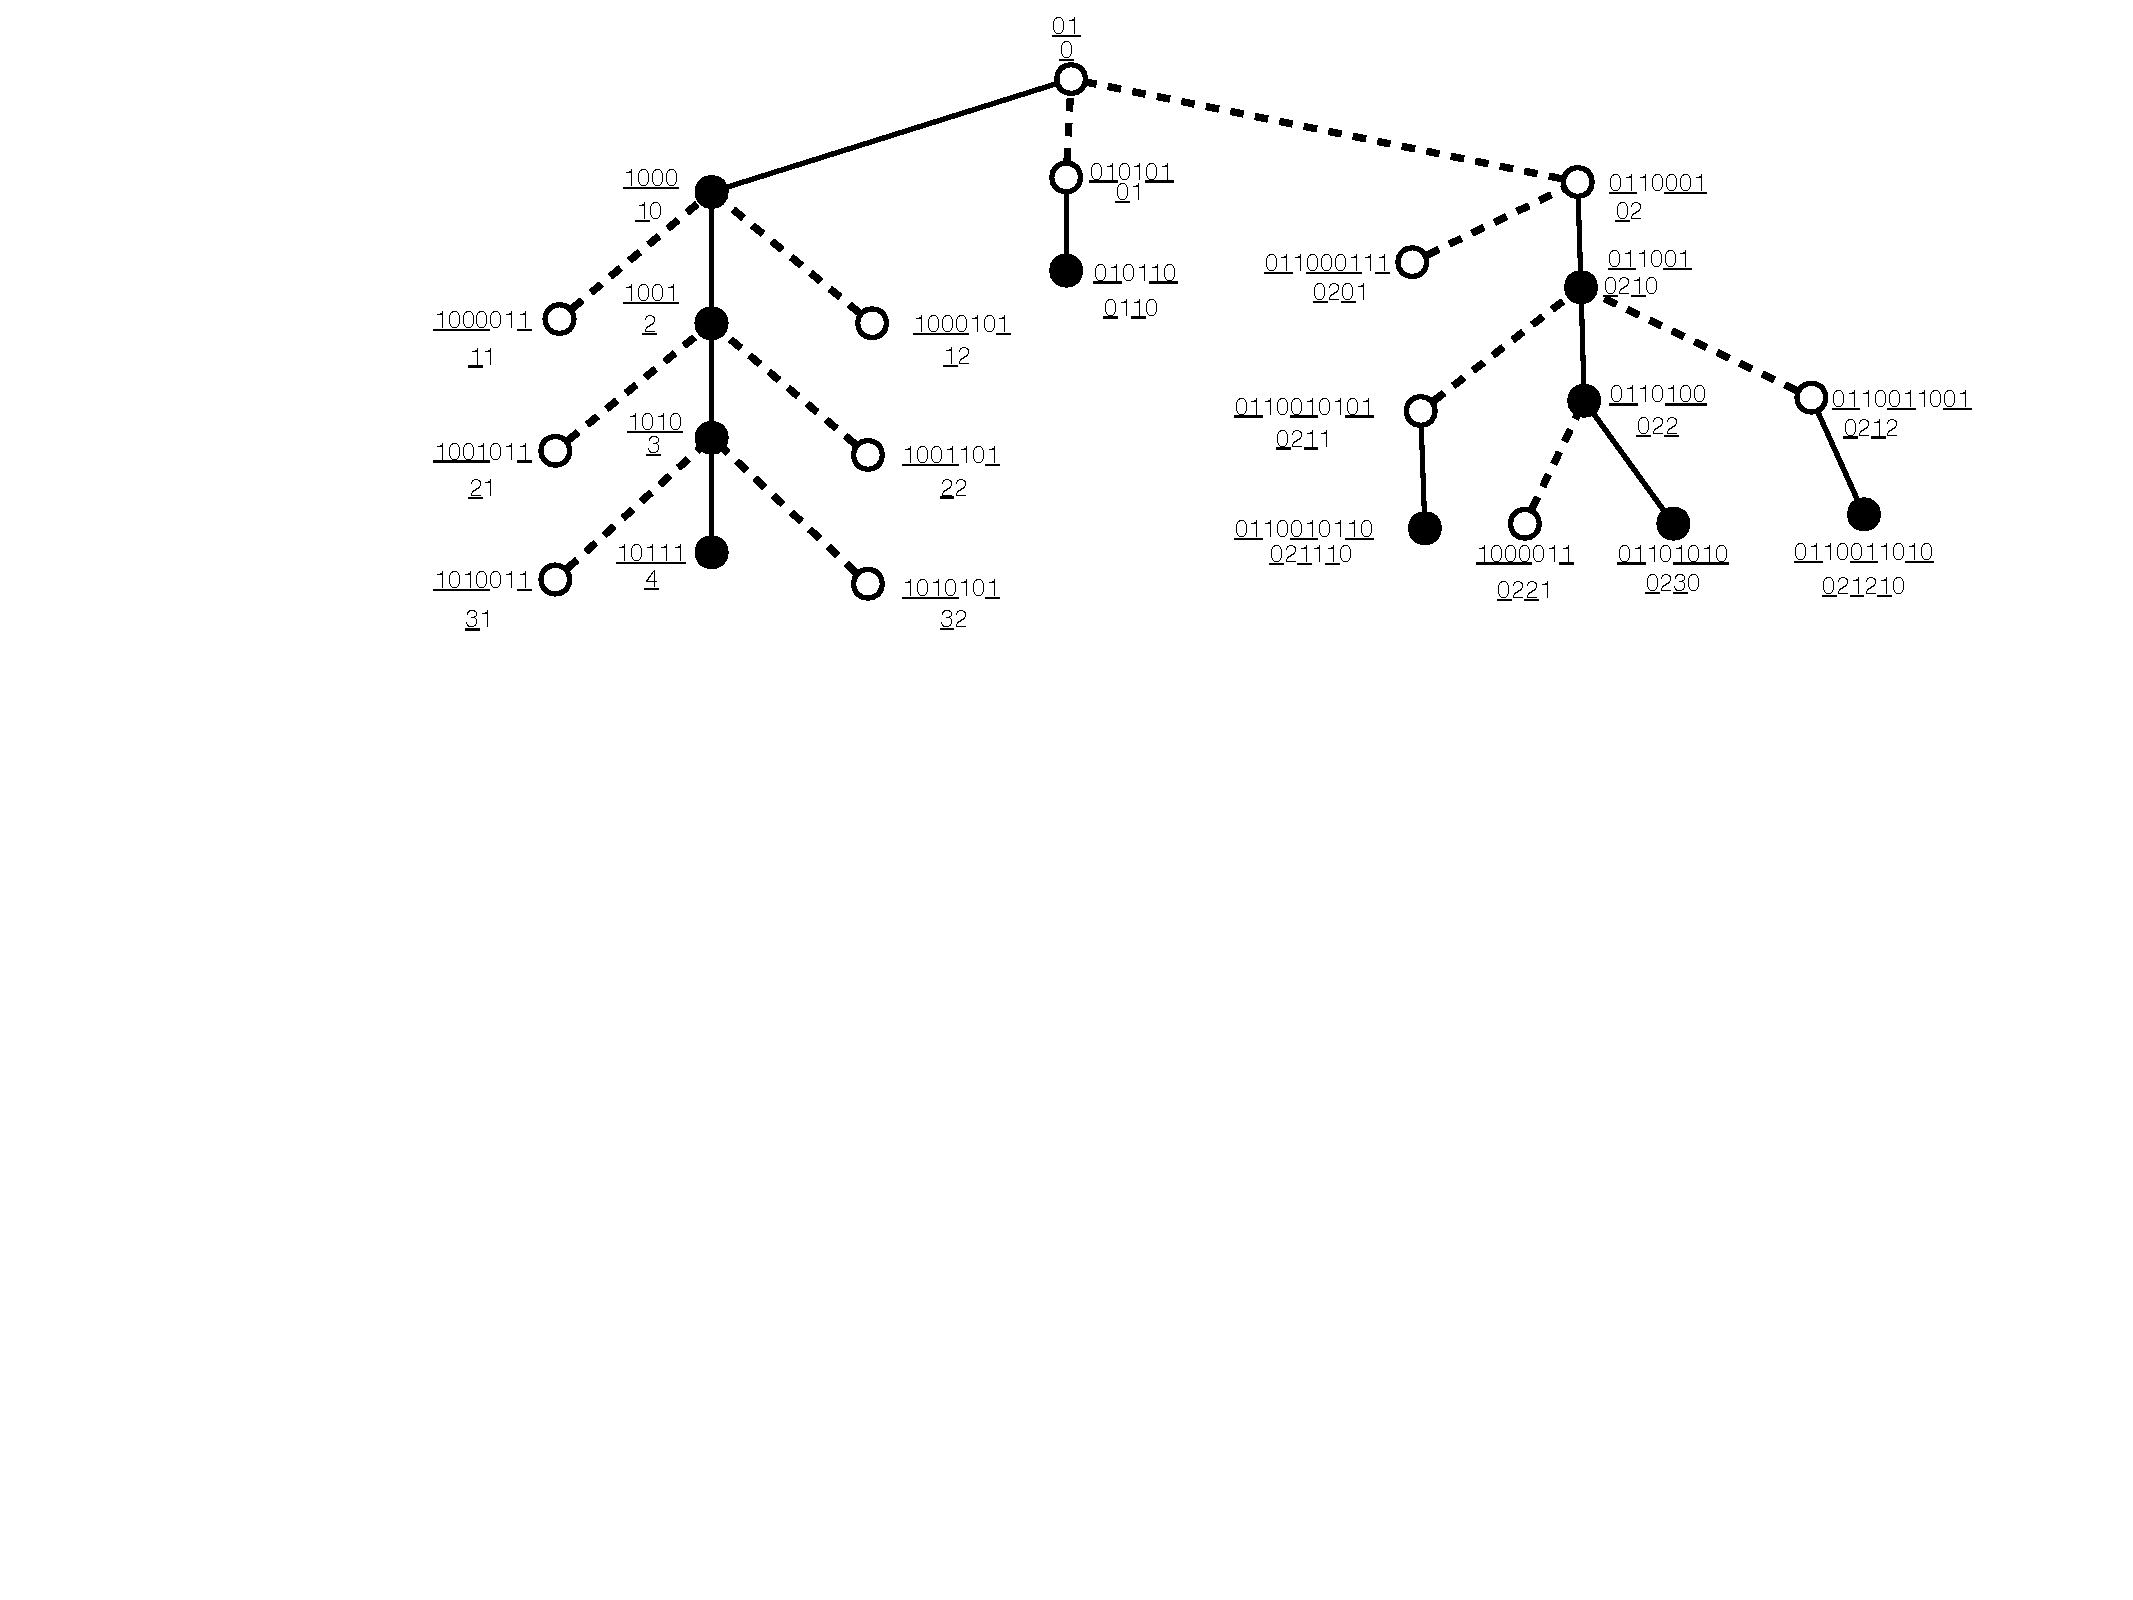
\includegraphics[width=120mm]{./Figures/Esbenscrazy.pdf}
				\caption{A tree with heavy (black) and light (white) nodes marked in the labeling scheme from Theorem~\ref{thm:nca-short} in binary on top and Theorem~\ref{NCA-fixed-upper} in decimal at the bottom. Both labels have their heavy sub-labels underlined.}
				\label{fig:NCAESBEN}
			\end{figure}
						
The labels constructed in Theorem~\ref{thm:nca-short}  can determine the first edge on the shortest path between the nodes queried. Therefore, using a slightly different decoder, we can construct a \routing labeling scheme (Section~\ref{section:Routing}).

The label size achieved in this method is at most $10 \log n$.
 \citeN{Green14} recently achieved an improved labeling scheme of size $3 \log n$ by replacing  Lemma~\ref{lemma:Gilbert} with a more compact  total order which allows for empty strings.

\paragraph{Labeling schemes with a query}
	  \citeN{Korman07K} extend  the definition of labeling scheme such that alongside the encoder and decoder, they define a \emph{query} function.
	Formally, given the labels $\la(u)$ and  $\la(v)$  of $u,v  \in  V $  outputs $Q(\la(u), \la(v))$ which is a node $ c \in V$.
	The decoder is free to use $c$ to compute the query.
	In this context, the authors proved that both  \NCAl and  \NCAf have a similar label size of  $O(\log n)$.
	The authors achieve similar label sizes for the functions \distance, \routing and \flow.
		
